Figure \ref{fig:Re40k_meshes} shows the series of adapted meshes obtained using the zonal-based refinement for $Re=40,000$. The corresponding VMS-based estimated error is also shown. As mentioned previously, mesh is refined in zones of high estimated error. 
Reduction in error can be seen as the mesh is refined.
Note that in-plane meshes from each series are shown in this figure.
Table \ref{table:adapt_mesh_details_Re40k} provides the number of elements for each of the 7 meshes.

\begin{table}[H]
	\centering
	\caption{Summary of meshes for adaptive LES at $Re=40,000$}
	\label{table:adapt_mesh_details_Re40k}
	\begin{tabular}{|l|c|c|c|c|}
		\hline
		Mesh   & No. of elements \\
		\hline
		M0\_nz25	& 774,525 \\
		\hline
		Mza1\_nz25	& 1,437,150 \\
		\hline		
		Mza1\_nz50 &  2,874,300 \\
		\hline
		Mza2\_nz50  &  7,164,600 \\
		\hline
		Mza2\_nz100  &  14,329,200 \\
		\hline
		Mza3\_nz50  &  18,286,100 \\
		\hline
		Mza3\_nz100  &  36,572,200 \\
		\hline
	\end{tabular}
\end{table}

\begin{figure}[H]
\centering

\begin{subfigure}[b]{0.475\textwidth}
\centering
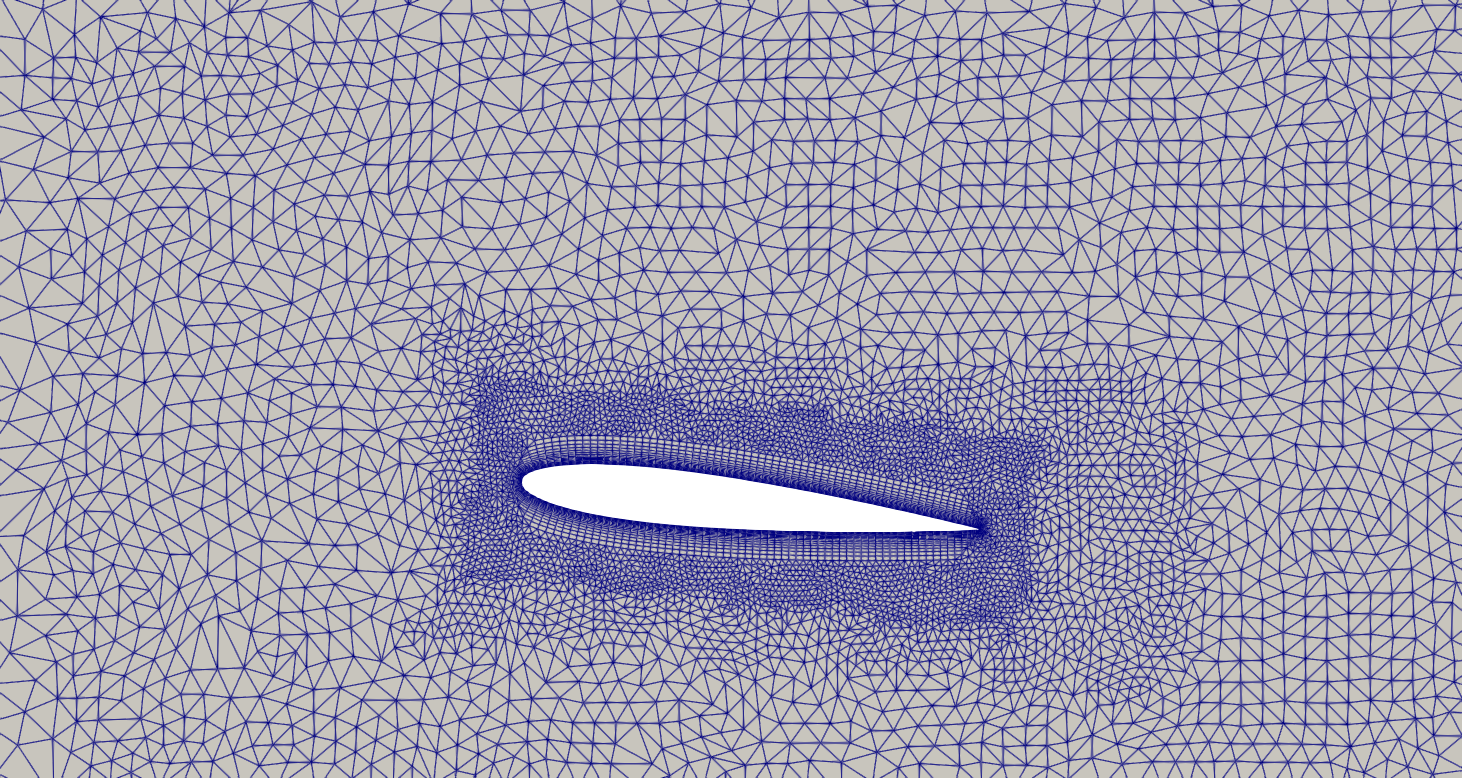
\includegraphics[width=1\textwidth]{figures/zonal_adapt_results/Mesh_and_error_plots/M0_inplane.png}
\caption{M0\_nz25 mesh}
\label{fig:zonal_M0_mesh}
\end{subfigure}
\begin{subfigure}[b]{0.475\textwidth}
\centering
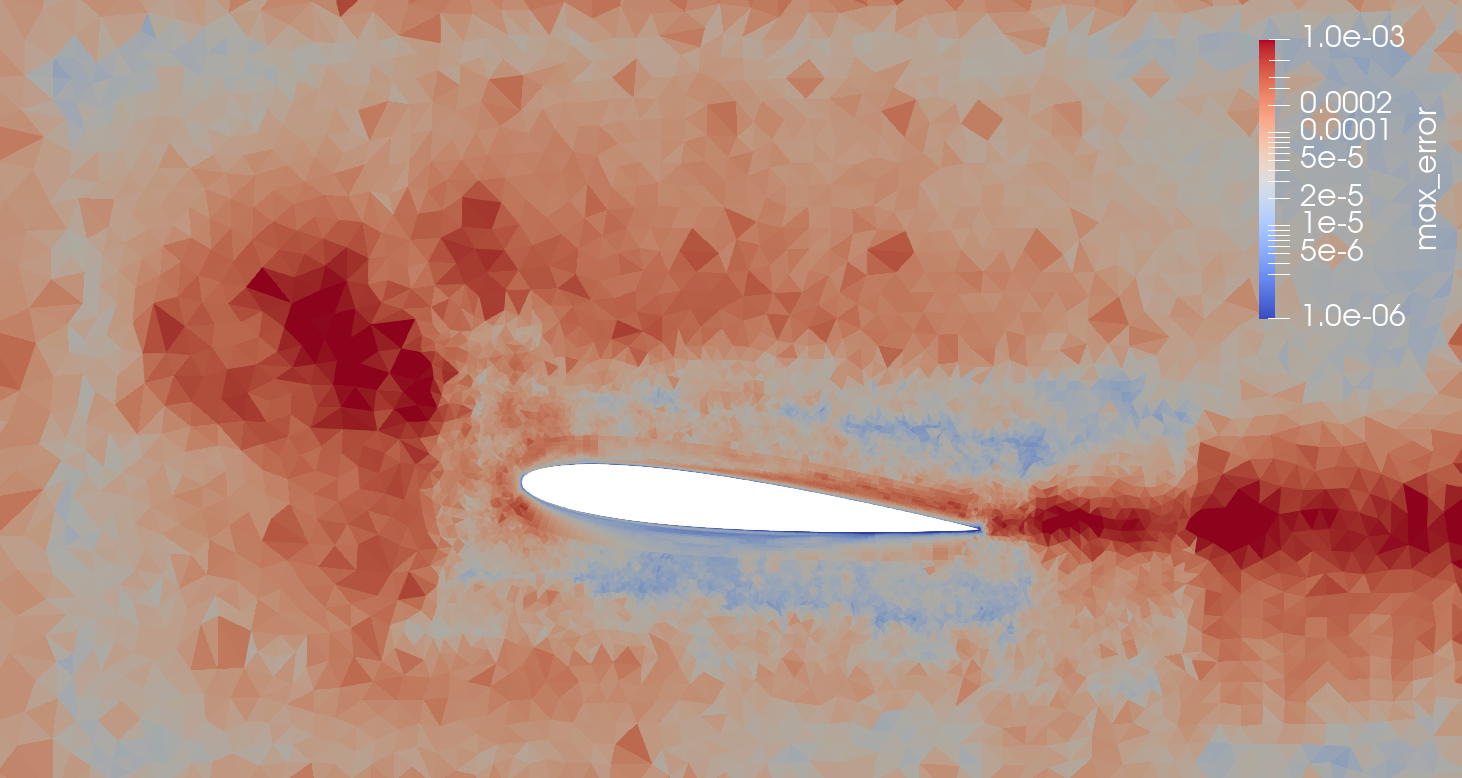
\includegraphics[width=1\textwidth]{figures/zonal_adapt_results/Mesh_and_error_plots/M0_error.png}
\caption{M0\_nz25 error field}
\label{fig:zonal_M0_error}
\end{subfigure}

\begin{subfigure}[b]{0.475\textwidth}
	\centering
	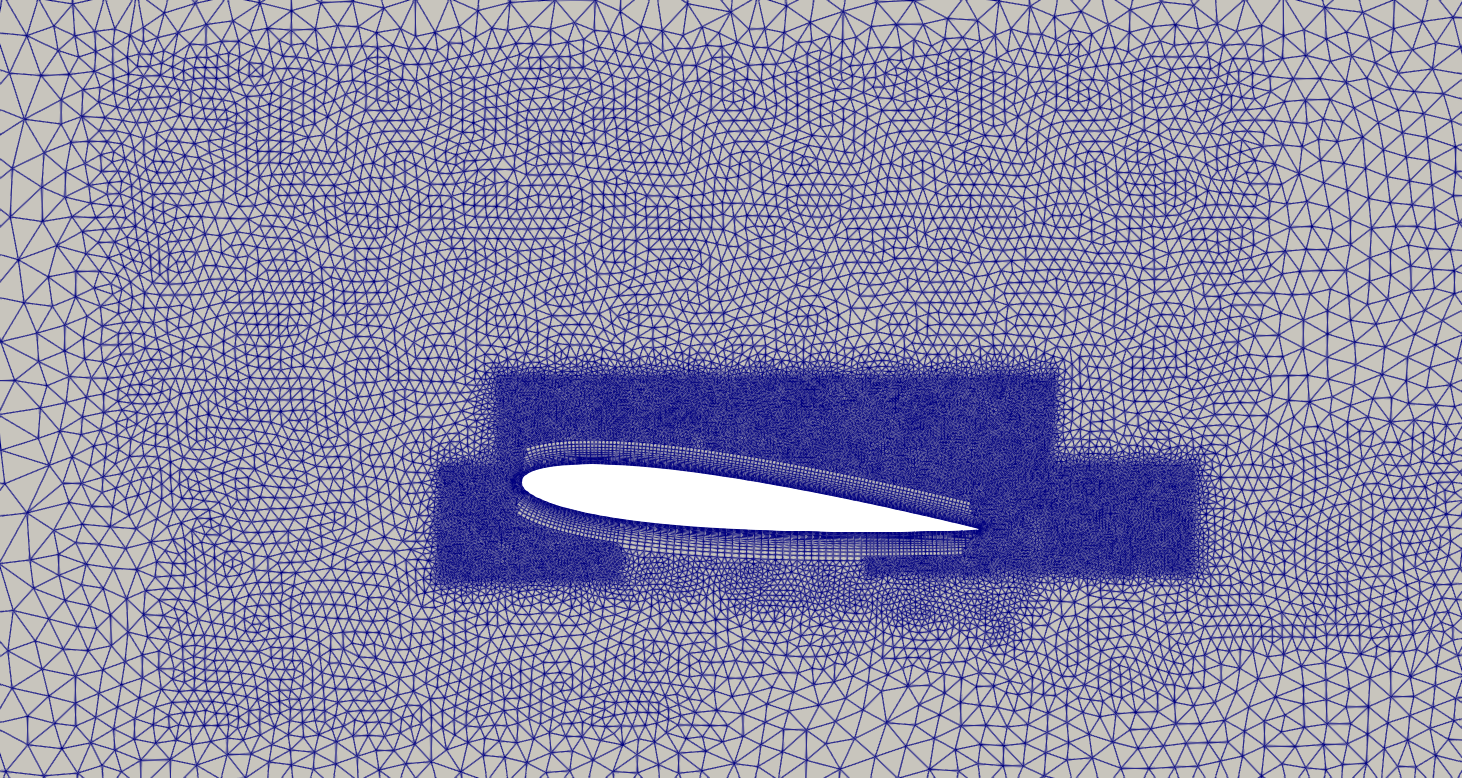
\includegraphics[width=1\textwidth]{figures/zonal_adapt_results/Mesh_and_error_plots/Mza1_inplane.png}
	\caption{Mza1\_nz25 mesh}
	\label{fig:zonal_Mza1_mesh}
\end{subfigure}
\begin{subfigure}[b]{0.475\textwidth}
	\centering
	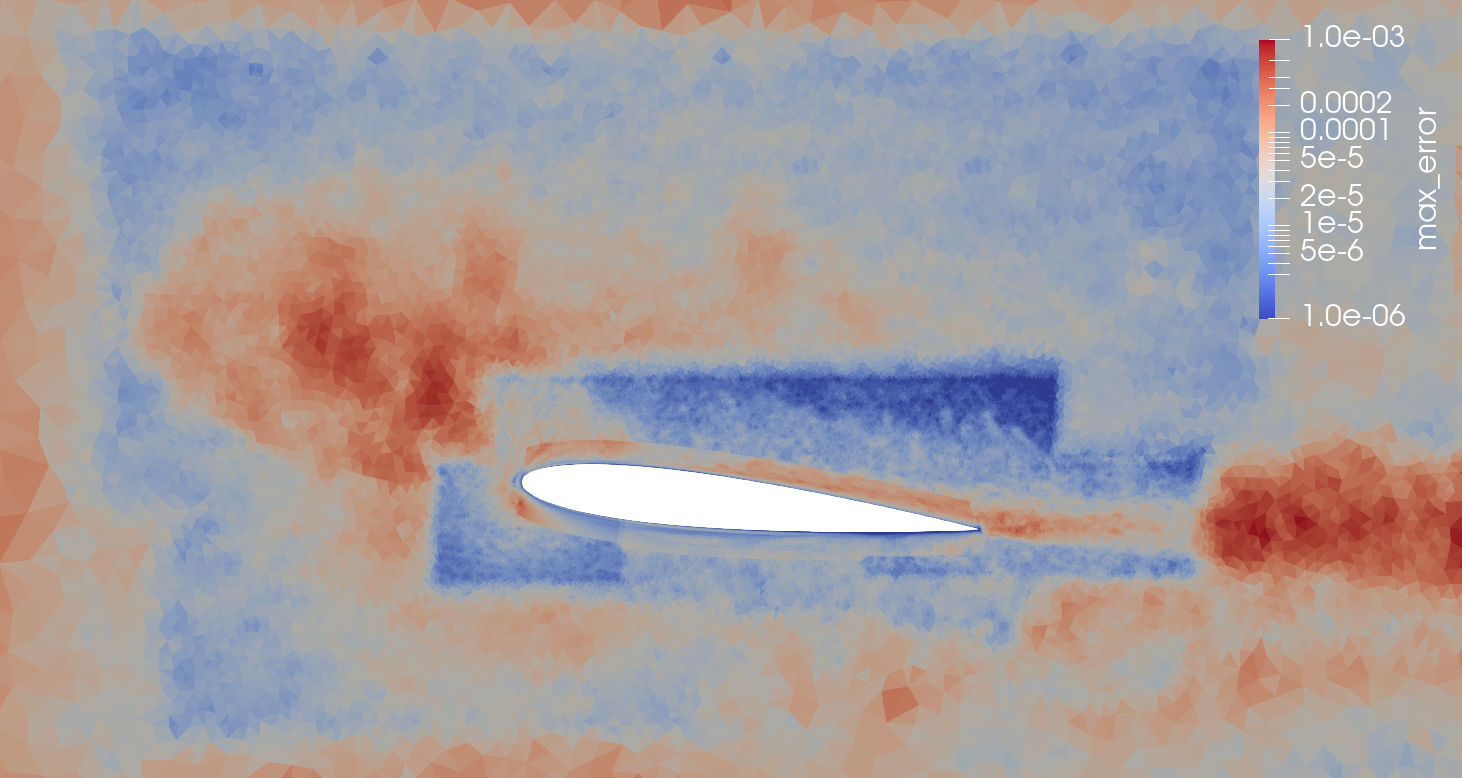
\includegraphics[width=1\textwidth]{figures/zonal_adapt_results/Mesh_and_error_plots/Mza1_error.png}
	\caption{Mza1\_nz25 error field}
	\label{fig:zonal_Mza1_error}
\end{subfigure}


\begin{subfigure}[b]{0.475\textwidth}
	\centering
	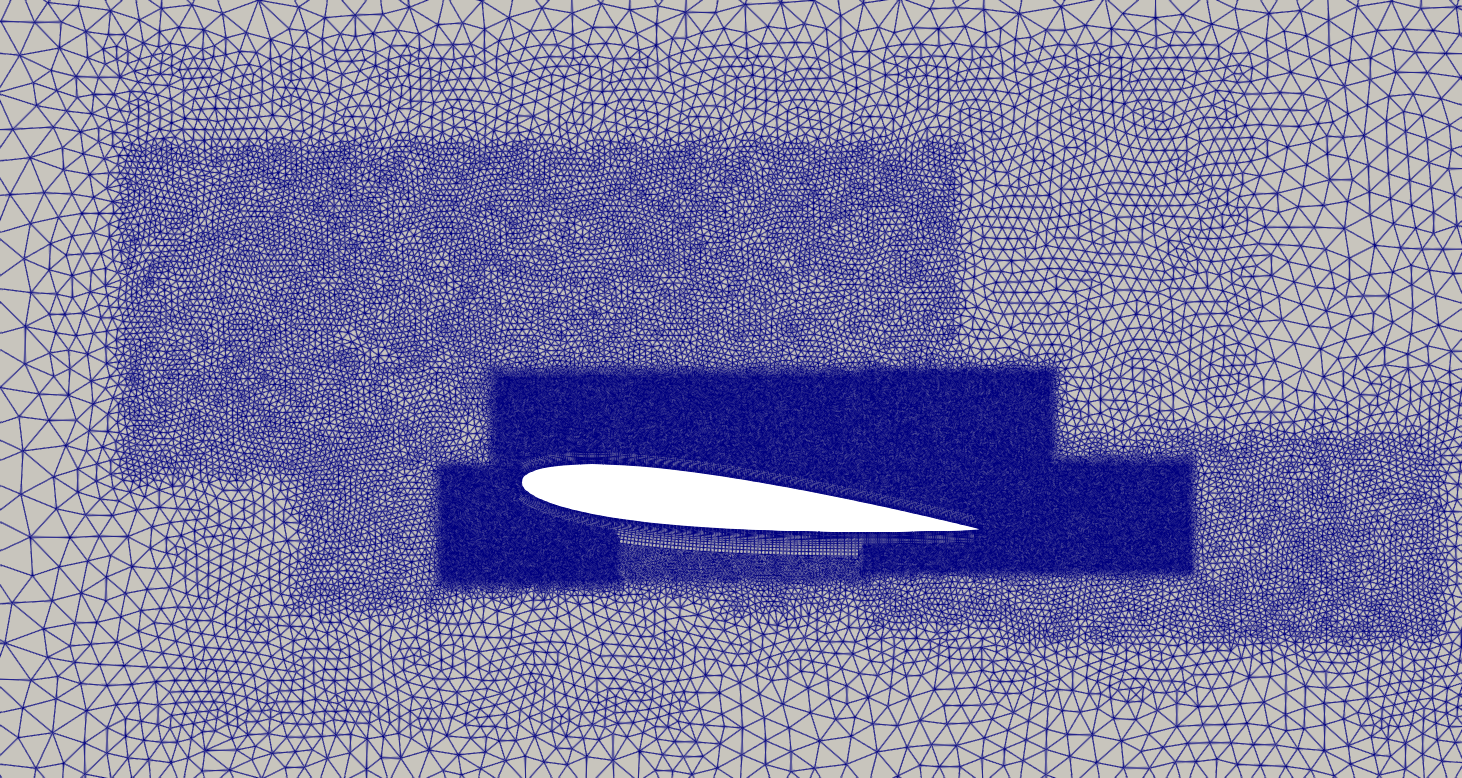
\includegraphics[width=1\textwidth]{figures/zonal_adapt_results/Mesh_and_error_plots/Mza2_inplane.png}
	\caption{Mza2\_nz50 mesh}
	\label{fig:zonal_Mza2_mesh}
\end{subfigure}
\begin{subfigure}[b]{0.475\textwidth}
	\centering
	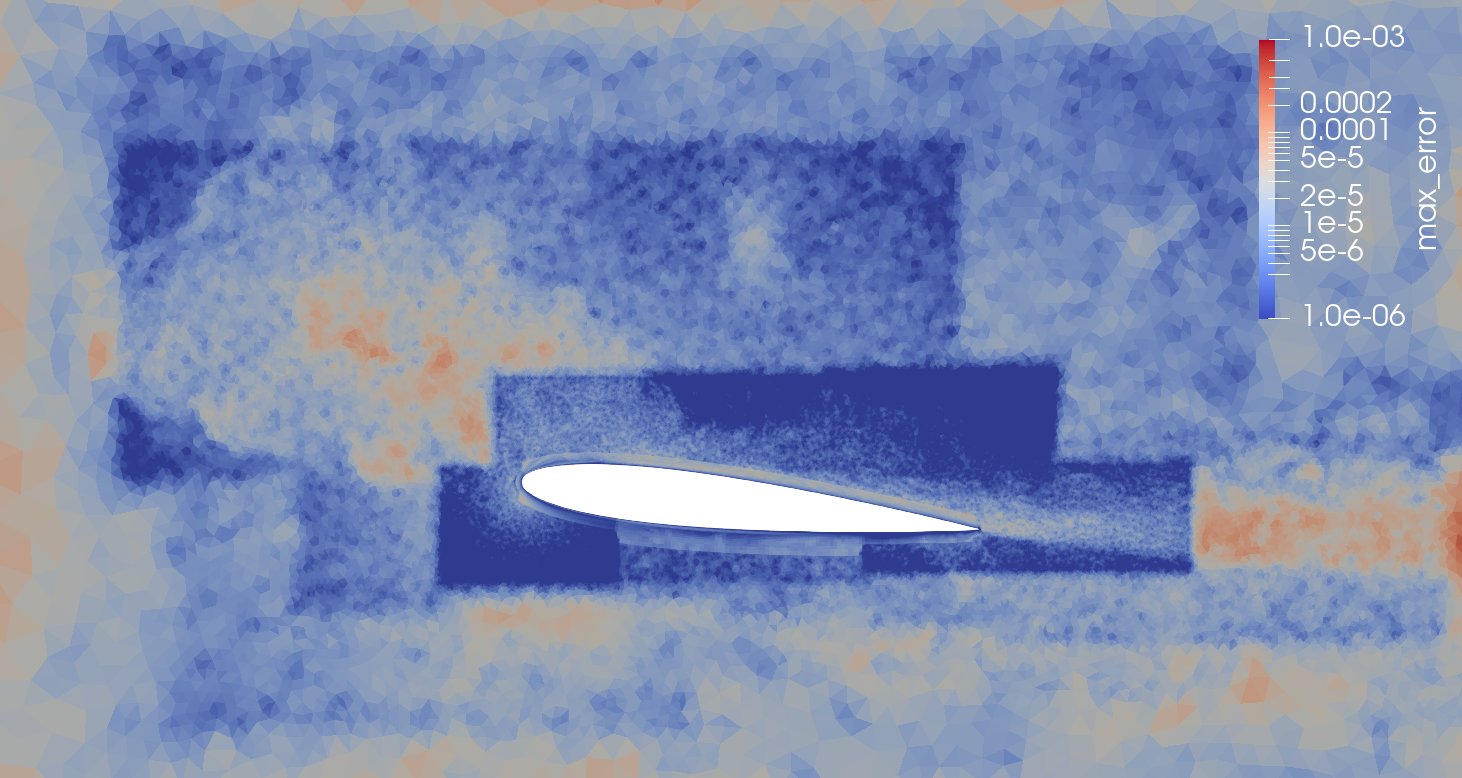
\includegraphics[width=1\textwidth]{figures/zonal_adapt_results/Mesh_and_error_plots/Mza2_error.png}
	\caption{Mza2\_nz50 error field}
	\label{fig:zonal_Mza2_error}
\end{subfigure}

\begin{subfigure}[b]{0.475\textwidth}
	\centering
	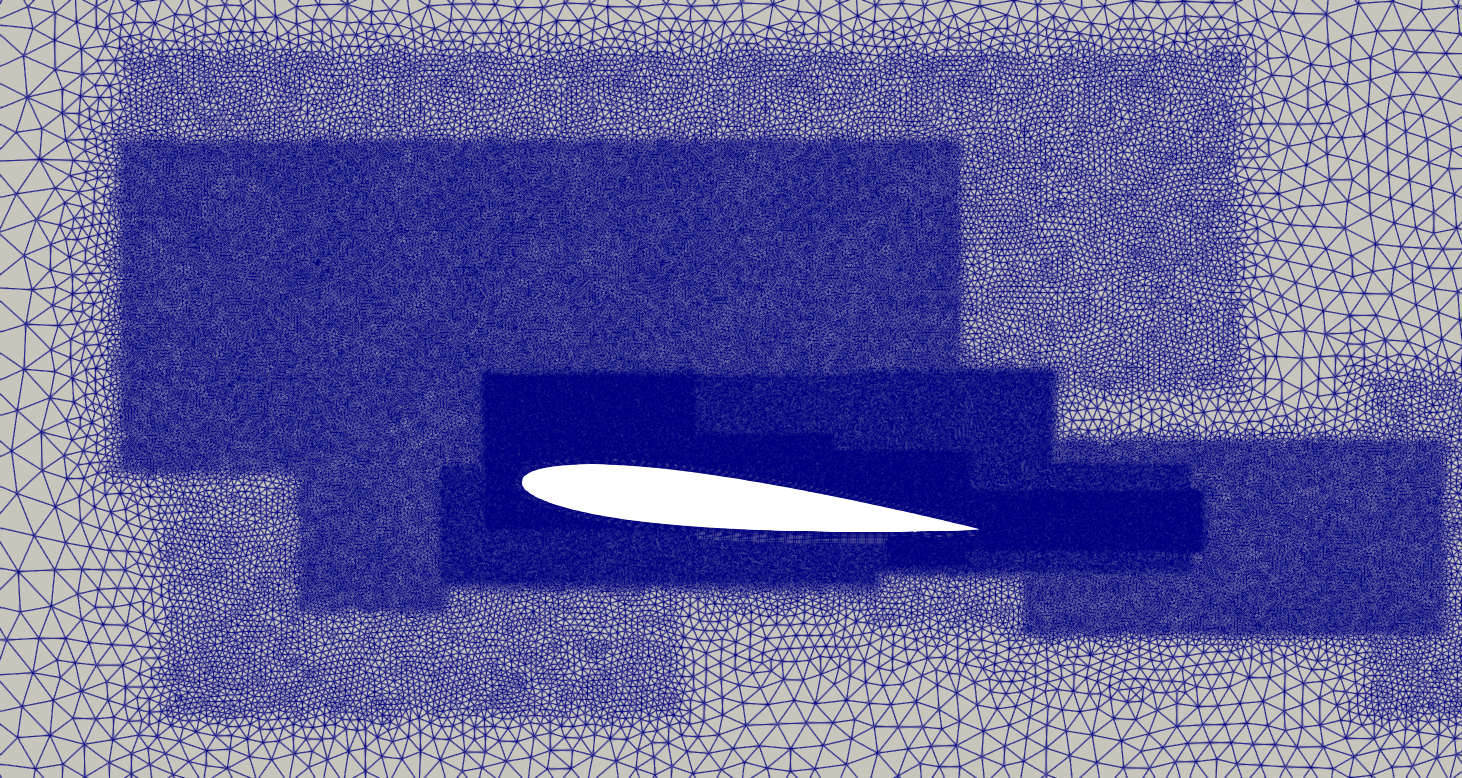
\includegraphics[width=1\textwidth]{figures/zonal_adapt_results/Mesh_and_error_plots/Mza3_inplane.png}
	\caption{Mza3\_nz50 mesh}
	\label{fig:zonal_Mza3_mesh}
\end{subfigure}
\begin{subfigure}[b]{0.475\textwidth}
	\centering
	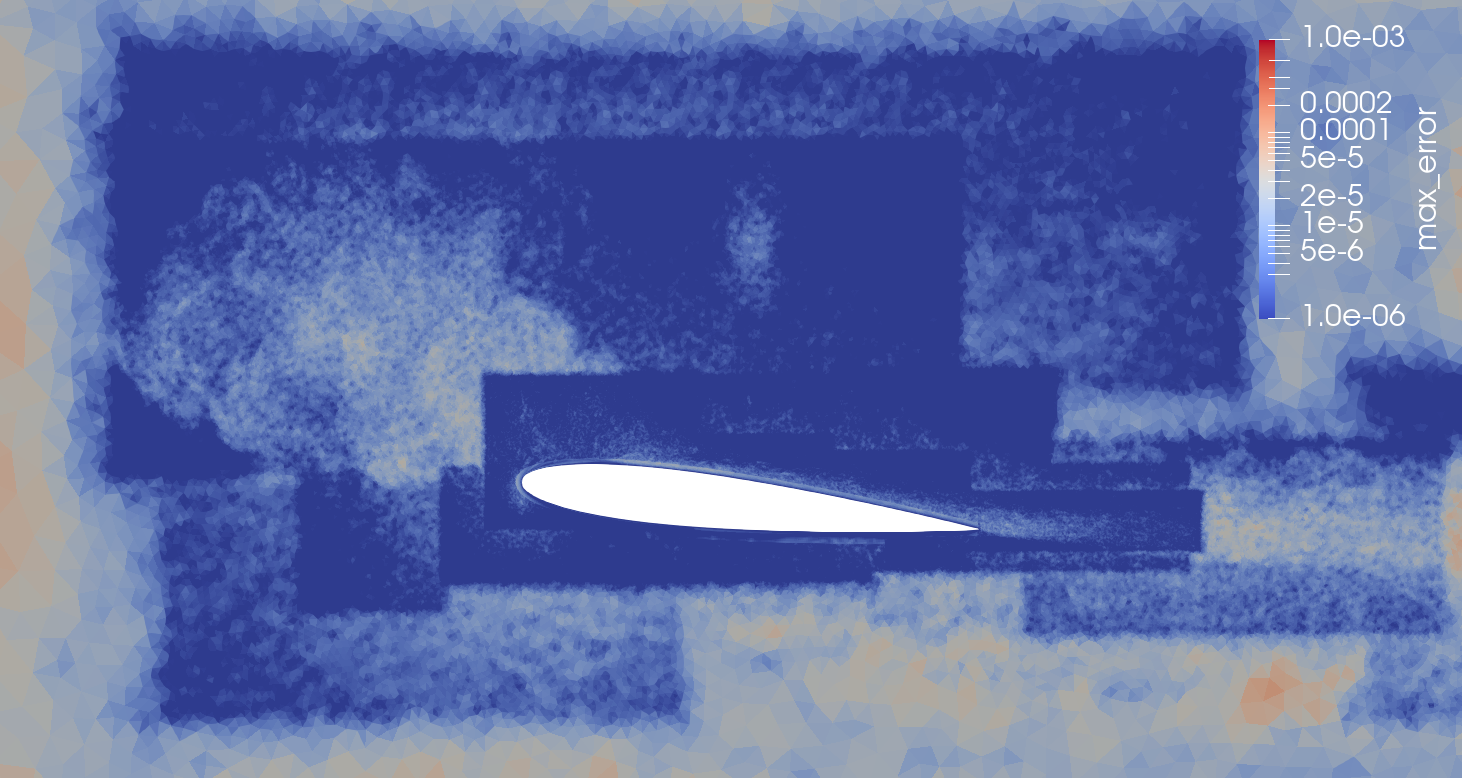
\includegraphics[width=1\textwidth]{figures/zonal_adapt_results/Mesh_and_error_plots/Mza3_error.png}
	\caption{Mza3\_nz50 error field}
	\label{fig:zonal_Mza3_error}
\end{subfigure}
\caption{Adaptive LES at $Re=40,000$: meshes and estimated error fields}
\label{fig:Re40k_meshes}
\end{figure}